\subsection{Measurement Setup}

The Goal of the measurements is to get an impression of the beamforming effect and compare it to the theoretical results from section \secref{sec:theory:beam}. As discussed in the previous sections the DAC and the software have some problems which could interfere with the result. Therefore the testsignal is generated by a waveform generator. Figure \ref{fig:meas:beam:setup} shows the measurement setup.
%
\begin{figure}
  \centering
  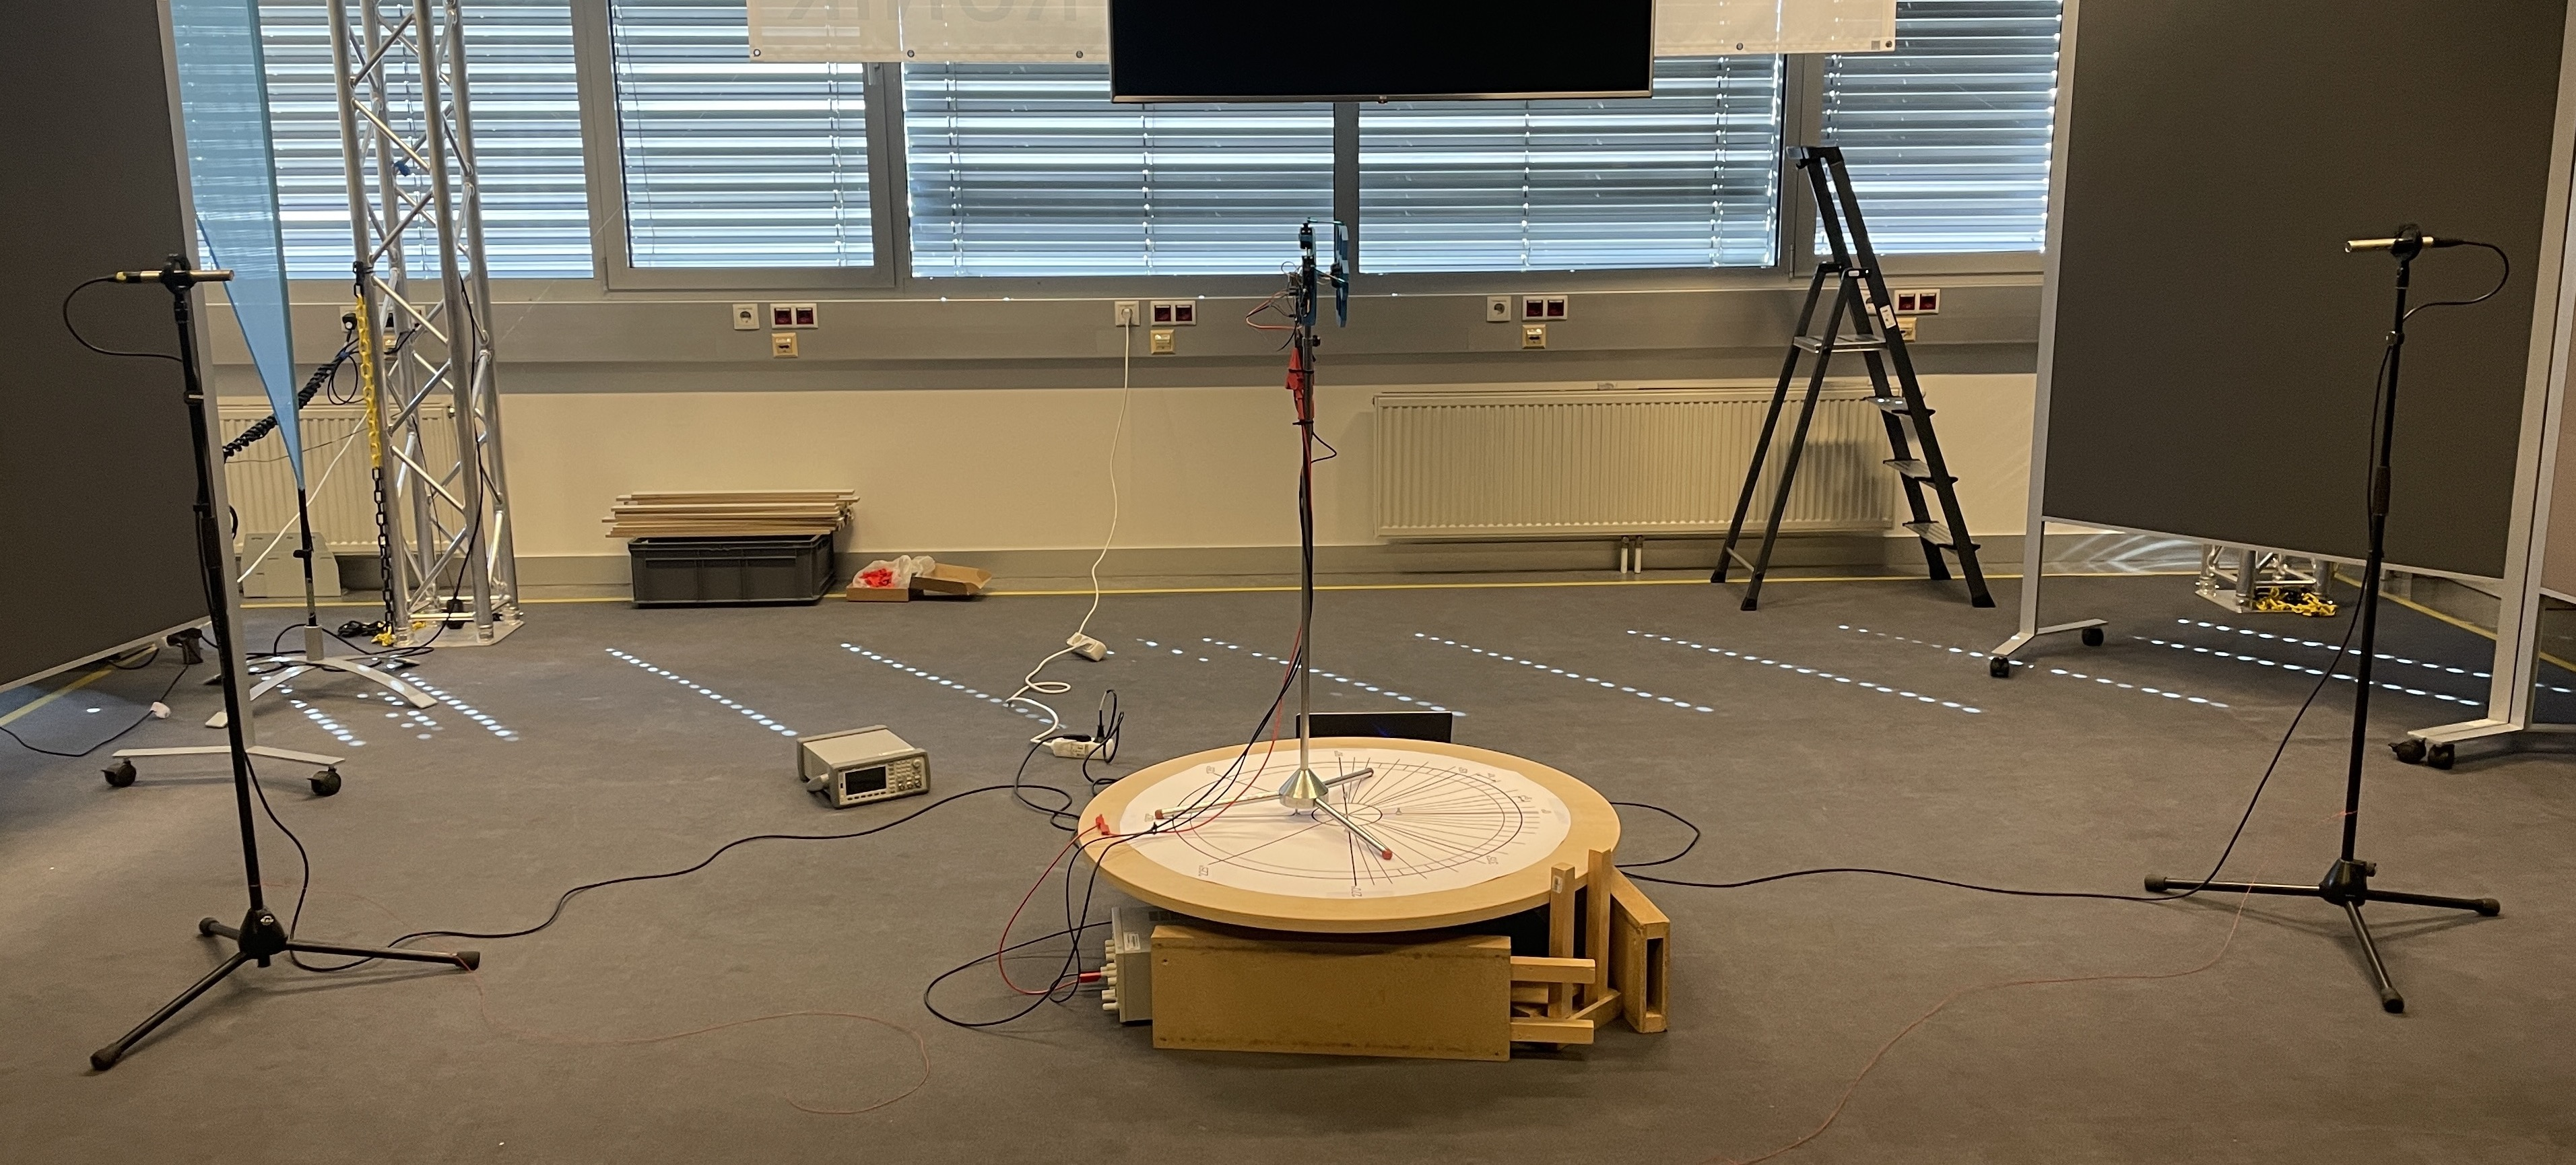
\includegraphics[height=\smallheight]{src/assets/pictures/measurements/beamforming_meas_setup.JPG}
  \caption{Measurement setup}\label{fig:meas:beam:setup}
\end{figure}
\p
The speaker is positioned on a rotating table to measure the audio for different angles. Two condenser microphones are positioned in front and behind the speaker. This halves the number of measurements needed for a full rotation. The audio is recorded with a \textbf{Zoom H5} audio interface.\p
%
AM and FM modulated sine signals with different frequencies between $0Hz$ and $20kHz$ are used to measure the behaviour of the speaker. The exact parameters are shown in table \ref{tab:meas:beam:params}. Each frequency is recorded for $7s$. Additionally, $3s$ of silence are recorded which can be used to filter noise.
%
\begin{table}
  \caption{Measurement parameters}\label{tab:meas:beam:params}
  \begin{tabular}{l||c|c|c}
    & \textbf{Modulation Depth} & \textbf{Carrier frequency}  & \textbf{Amplitude}\\
    \hline
    \textbf{AM} & $0.8$         & $40kHz$                     & $2V$ \\
    \textbf{FM} & $5kHz$        & $40kHz$                     & $2V$ \\
  \end{tabular}
\end{table}